\documentclass{report}
\usepackage[spanish]{babel}
\usepackage[utf8]{inputenc}
\usepackage{graphicx, longtable, float, titlesec, hyperref, enumitem, dingbat}
\usepackage[dvipsnames]{xcolor}
\usepackage[margin=2.75cm]{geometry}

\hypersetup{
    hidelinks = true
}

\titleformat{\chapter}[display]
  {\normalfont\bfseries}{}{0pt}{\Huge\thechapter.\space}

\titleformat{name=\chapter,numberless}[display]
  {\normalfont\bfseries}{}{0pt}{\Huge}

\titlespacing*{\chapter}{0pt}{-50pt}{20pt}


\begin{document}
    \begin{titlepage}
        \centering
        
\includegraphics[width=0.6\textwidth]{./img/logo.jpg}\\
        \vspace{1cm}
        \LARGE Gestión de proyectos\\
        \vspace{0.5cm}
        \Large Ingeniería Informática de Gestión y Sistemas de Información\\
        \vspace{3cm}
        \Huge PromoIng Civil UPV/EHU\\
        \huge XabierCorp\\
        \vspace{2.5cm}
        \Large Autor:\\
        \vspace{0.2cm}
        \large Xabier Gabiña\\
        \large Endika Postigo\\
        \large Xabier Badiola\\
        \large Ander Gorocica\\
        \large Asier Larrazabal\\
        \large Pablo Leclercq\\
        \vfill
        \today
    \end{titlepage}
    \tableofcontents
    \listoffigures
    \listoftables
    \chapter{Introducción}
        \section{Introducción del Proyecto}
            \paragraph*{}
            Este documento detalla la propuesta solicitada por la persona responsable para promocionar las titulaciones de la Escuela de Ingeniería de Bilbao para el desarrollo de un vídeo promocional y una plataforma web. El objetivo es destacar la titulación de Ingeniería Civil, subrayando sus beneficios únicos, infraestructura y oportunidades. Además, la plataforma web mostrará un video sobre dicha titulación y servirá para recoger datos de contacto de estudiantes potenciales e incluirá la organización de un sorteo entre los participantes, ofreciendo material corporativo de la universidad como incentivo.
        \section{Propósito del Proyecto}
            \paragraph*{}
            El propósito de este proyecto es elaborar un video promocional y desarrollar una página web que exponga de manera atractiva y concisa las características de la titulación de Ingeniería Civil de la Escuela de Ingeniería de Bilbao, incluyendo los objetivos educativos, infraestructura, y las oportunidades de prácticas y proyectos. Proporcione una manera directa y sencilla para que los interesados dejen sus datos de contacto a través de la plataforma web, facilitando así la recolección de información. Además, se incluirá en la plataforma un sorteo de material corporativo de la universidad entre los participantes que completen el formulario de contacto.
        \section{Asociaciones y Ámbito de Aplicación}
            \paragraph*{}
            Este proyecto se realiza a petición de la persona encargada de la promoción de las titulaciones en la Escuela de Ingeniería de Bilbao y está diseñado para soportar la promoción de sus programas académicos. La plataforma web contendrá el video promocional y será accesible en todos los navegadores, asegurando que el público objetivo pueda acceder fácilmente a la información y participar en el sorteo.
        \section{Contexto de Negocio}
            \paragraph*{}
            El proyecto se enfoca en proporcionar herramientas digitales promocionales específicas para la Escuela de Ingeniería de Bilbao, orientadas a atraer a estudiantes de último año de bachillerato y profesionales jóvenes interesados en las titulaciones ofrecidas, en nuestro caso la Ingeniería Civil.. Responde a la necesidad de la escuela de resaltar los puntos fuertes de sus programas y de facilitar la recogida de datos de posibles candidatos, promoviendo así un mayor interés tanto a nivel nacional como internacional. La inclusión de un sorteo busca añadir un incentivo adicional para el registro de datos en la plataforma.
        \section{Definiciones, Acrónimos y Abreviaturas}
            \paragraph*{}
            \begin{itemize}
                \item \textbf{UPV/EHU:} Universidad del País Vasco/Euskal Herriko Unibertsitatea.
                \item \textbf{DOP:} Documento de Planificación.
                \item \textbf{PromoIng Civil UPV/EHU:} Proyecto de promoción de la titulación de Ingeniería Civil de la UPV/EHU.
                \item \textbf{SMART:} Es un acrónimo en inglés que se utiliza para definir objetivos específicos, medibles, alcanzables, relevantes y con un tiempo determinado.
            \end{itemize}
    \chapter{Descripción del proyecto}
        \section{Descripción del Proyecto}
            \paragraph*{}
            El proyecto PromoIng Civil UPV/EHU es una iniciativa encargada por la persona responsable de promocionar las titulaciones de la Escuela de Ingeniería de Bilbao, perteneciente a la Universidad del País Vasco / Euskal Herriko Unibertsitatea (UPV/EHU). Este proyecto integra el desarrollo de un video promocional y una plataforma web, destinados a resaltar las ventajas y oportunidades de estudiar la titulación de Ingeniería Civil en una de las instituciones más reconocidas de la región. Un aspecto distintivo de la plataforma web será la inclusión de un sorteo entre los interesados que proporcionen sus datos, ofreciendo material corporativo de la universidad como premio.
        \section{Problema que Resuelve}
            \paragraph*{}
            En un contexto de creciente competencia educativa, la UPV/EHU enfrenta el reto de mantener y diversificar su matrícula. El proyecto PromoIng Civil UPV/EHU surge como respuesta a la necesidad de mejorar la visibilidad y efectividad de las comunicaciones sobre la titulación de Ingeniería Civil. Al presentar de manera más atractiva esta titulación a potenciales estudiantes, tanto a nivel local como internacional, y facilitar la recopilación de datos de los interesados, el proyecto busca fortalecer la comunidad universitaria.
        \section{Valor del Desarrollo}
            \paragraph*{}
            La importancia de desarrollar PromoIng Civil UPV/EHU reside en varios aspectos clave:
            \begin{itemize}
                \item \textbf{Fortalecimiento de la Identidad Institucional:} La asociación directa del proyecto con la UPV/EHU destaca el prestigio y la calidad de la universidad, reforzando su imagen como líder en la educación en ingeniería.
                \item \textbf{Mejora de la Estrategia de Comunicación:} Mediante el uso de herramientas digitales y contenido atractivo, el proyecto facilita la comunicación de las características únicas y beneficios de la titulación de Ingeniería Civil, resonando con las expectativas de los estudiantes actuales.
                \item \textbf{Aumento de la Visibilidad y Alcance:} Se busca mejorar la posición de la Escuela de Ingeniería de Bilbao y de la UPV/EHU en el ámbito nacional e internacional como referentes en estudios de ingeniería.
                \item \textbf{Optimización del Proceso de Reclutamiento:} La plataforma web ofrecerá un canal directo y eficiente para interactuar con los interesados, facilitando el proceso de admisión y aumentando las tasas de conversión de interesados a estudiantes matriculados.
            \end{itemize}
            En conclusión, el proyecto PromoIng Civil UPV/EHU no solo eleva la visibilidad de una titulación específica sino que también contribuye al fortalecimiento de la marca UPV/EHU como institución líder en educación superior, especialmente en ingeniería. Este esfuerzo se alinea con los objetivos estratégicos de la universidad de atraer talento y fomentar la innovación y la excelencia académica en el País Vasco y más allá, incluyendo el sorteo como un incentivo adicional para la participación en la plataforma web.
    \chapter{Objetivos del proyecto}
        \section{Desarrollo del Proyecto PromoEng Civil UPV/EHU}
            \paragraph*{}
            El proyecto PromoEng Civil UPV/EHU tiene como fin el desarrollo de una plataforma web accesible y la producción de un video promocional integrado en dicha plataforma. Este enfoque busca maximizar la visibilidad y el atractivo de la titulación de Ingeniería Civil de la Escuela de Ingeniería de Bilbao, UPV/EHU. Los objetivos son:
            \begin{itemize}
                \item Desarrollar una plataforma web accesible y producir un video promocional de 3 minutos para aumentar la visibilidad y el atractivo de la titulación de Ingeniería Civil de la Escuela de Ingeniería de Bilbao, UPV/EHU.
                \item Producir un video que incluya testimonios, vistas de instalaciones y descripciones de oportunidades profesionales, integrándolo de manera destacada en la plataforma web para asegurar su visibilidad. La plataforma debe incluir secciones para información del programa, contacto, y el video promocional, además de un sistema para la recopilación y gestión eficiente de datos de contacto.
                \item Utilizar el video como herramienta clave para aumentar el interés por la titulación, complementando la información disponible en la plataforma web. Proporcionar un recurso completo y accesible para aumentar las solicitudes de información y admisión.
                \item Completar el video y su integración en la plataforma web en un plazo de 4 meses desde el inicio del proyecto. Finalizar el desarrollo, pruebas y lanzamiento de la plataforma web en el mismo período. Completar las pruebas y ajustes necesarios antes del lanzamiento oficial de la plataforma y el video.
            \end{itemize}
    \chapter{Arquitectura}
        \paragraph*{}
        Hemos decidido utilizar una arquitectura Web y una plataforma llamada Docker para realizar este proyecto. Docker sigue una estructura basada en contenedores y los utiliza para encapsular y distribuir aplicaciones. Dentro de este proyecto vamos a incluir un contenedor para desplegar la página web, otro para el reproductor de youtube y otro para el formulario de Google Forms, que este tendrá una base de datos. La página web tendrá la siguiente estructura:
        \begin{itemize}
            \item Un video donde resume la información que contiene la pantalla de inicio.
            \item Información relevante sobre el grado de Ingeniería Civil, por ejemplo, las salidas que tiene el grado, los puestos de trabajo en los que pueden trabajar en un futuro al terminarlo, opiniones sobre los alumnos que han cursado este grado.
            \item Un formulario donde se recoge información de interés sobre los interesados en cursar el grado, por ejemplo, los estudios actuales, la edad, el curso que está realizando, si está realizando un bachiller o una FP, quien rellena la encuesta (familiar, el propio alumno…). Además, se van a sortear dos mochilas de la UPV/EHU entre las personas que rellenen la encuesta (el sorteo se realizará de manera aleatoria y manual).
        \end{itemize}
        
        Dentro de la base de datos de Google Forms se guardará toda la información relativa a los usuarios que rellenen la encuesta de la página web.\\
        \clearpage
        La arquitectura de este sistema web funciona de la siguiente manera:
        \begin{itemize}
            \item El usuario accede a la página web desde su navegador.
            \item La página web esta desplegada en un cluster Kubernetes corriendo en Google Cloud que asegura la disponibilidad de la página web.
            \item Dicho cluster esta corriendo un 'Pod' con la imagen Docker de la página web de esta forma se consigue que la web sea facilmente escalable.
            \item La página web carga elementos de Youtube y Google Forms mediante iFrames además de los elementos propios y los muestra mediante el navegador al usuario.
        \end{itemize}
        \begin{figure}[H]
            \centering
            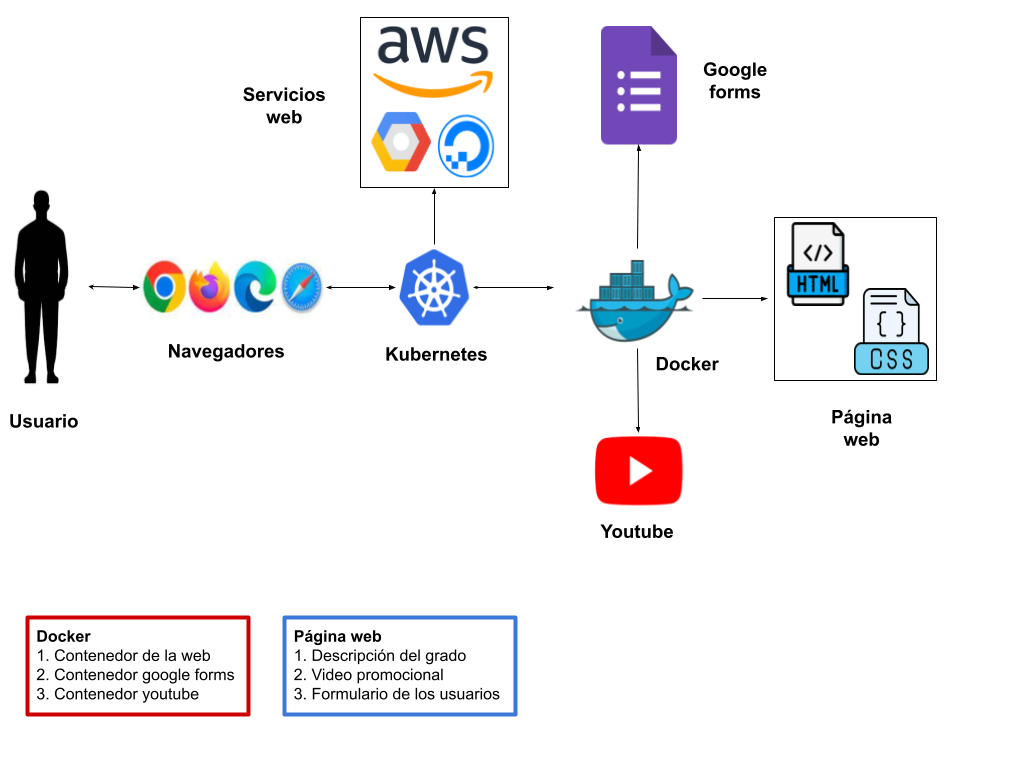
\includegraphics[width=0.8\textwidth]{./img/arquitectura.png}
            \caption{Arquitectura del sistema}
        \end{figure}
    \chapter{Herramientas}
        \section*{Git}
            Git es un sistema de control de versiones distribuido de código abierto y gratuito diseñado para manejar todo, desde proyectos pequeños hasta muy grandes, con velocidad y eficiencia. Lo utilizaremos para controlar las versiones del código fuente de la página web.
        \section*{GitHub}
            GitHub es una plataforma de desarrollo colaborativo para alojar proyectos utilizando el sistema de control de versiones Git. Lo utilizaremos para alojar el código fuente de la página web junto con la documentación del proyecto
        \section*{LibreOffice}
            LibreOffice es una suite ofimática de codigo abierto que incluye programas para el procesamiento de texto, hojas de cálculo, presentaciones, bases de datos y dibujos. Lo utilizaremos para la redacción de la documentacion.
        \section*{LaTeX}
            LaTeX es un sistema de composición de textos, orientado a la creación de documentos escritos que presenten una alta calidad tipográfica. Lo utilizaremos para la redacción de la documentacion.
        \section*{Apache HTTP Server}
            Apache HTTP Server es un servidor web HTTP de código abierto multiplataforma que nos servira para desarrollar nuestra página web.
        \section*{Docker}
            Docker es un proyecto de código abierto que automatiza el despliegue de aplicaciones dentro de contenedores de software, proporcionando una capa adicional de abstracción y automatización de virtualización a nivel de sistema operativo en Linux. Utilizaremos Docker para desplegar nuestra página web en un contenedor.
        \section*{Kubernetes}
            Kubernetes es un sistema de código abierto para la automatización del despliegue, escalado y manejo de aplicaciones en contenedores originalmente diseñada por Google. La usaremos para desplegar nuestra imagen Docker en un cluster de Google Cloud.
        \section*{VSCode}
            Visual Studio Code es un editor de código fuente desarrollado por Microsoft para Windows, Linux y macOS. Lo utilizaremos para la programación de la página web.
        \section*{Google Cloud Platform}
            Google Cloud Platform es una suite de servicios en la nube que se ejecutan en la misma infraestructura que Google utiliza internamente para sus productos de usuario final, como Google Search y YouTube. Junto con un conjunto de herramientas de administración, seguridad y desarrollo, Google Cloud Platform proporciona una serie de servicios como es el caso de Kubernete Engine.
        \section*{Google Forms}
            Google Forms es una herramienta de Google que nos permite crear encuestas y cuestionarios de manera sencilla y rápida. Lo utilizaremos para recoger información de los interesados en cursar el grado de Ingeniería Civil.
        \section*{Youtube}
            Youtube es una plataforma de videos en la que los usuarios pueden subir, compartir y ver videos. Lo utilizaremos para alojar el video promocional de la página web.
        \section*{GanttProject}
            GanttProject es una herramienta de código abierto para la creación de diagramas de Gantt y la gestión de proyectos. Lo utilizaremos para la planificación temporal del proyecto.
    \chapter{Alcance del proyecto}
        \section{Ciclo de vida}
            \paragraph*{}
            Para el desarrollo de este proyecto hemos decidido utilizar un ciclo de vida adaptativo o ágil. Las actividades de desarrollo se completarán una tras otra. Las actividades de prueba solo ocurrirán después de que todas las actividades de desarrollo se hayan completado.  Tomaremos el siguiente orden de ciclo:
            \begin{figure}[H]
                \centering
                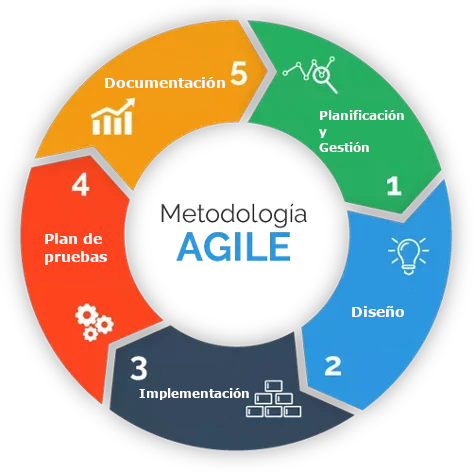
\includegraphics[width=0.5\textwidth]{./img/ciclo_vida.png}
                \caption{Ciclo de vida del proyecto}
            \end{figure}
            Una de las razones por la que hemos elegido este modelo de ciclo de vida es que los equipos trabajan en ciclos cortos de desarrollo y además se adaptan a los cambios propuestos por el cliente a medida que surgen, pudiendo variar así la planificación y la gestión del proyecto en cualquier momento.
        \clearpage
        \section{Fases del proyecto}
            \textbf{EDT}
            \begin{figure}[H]
                \centering
                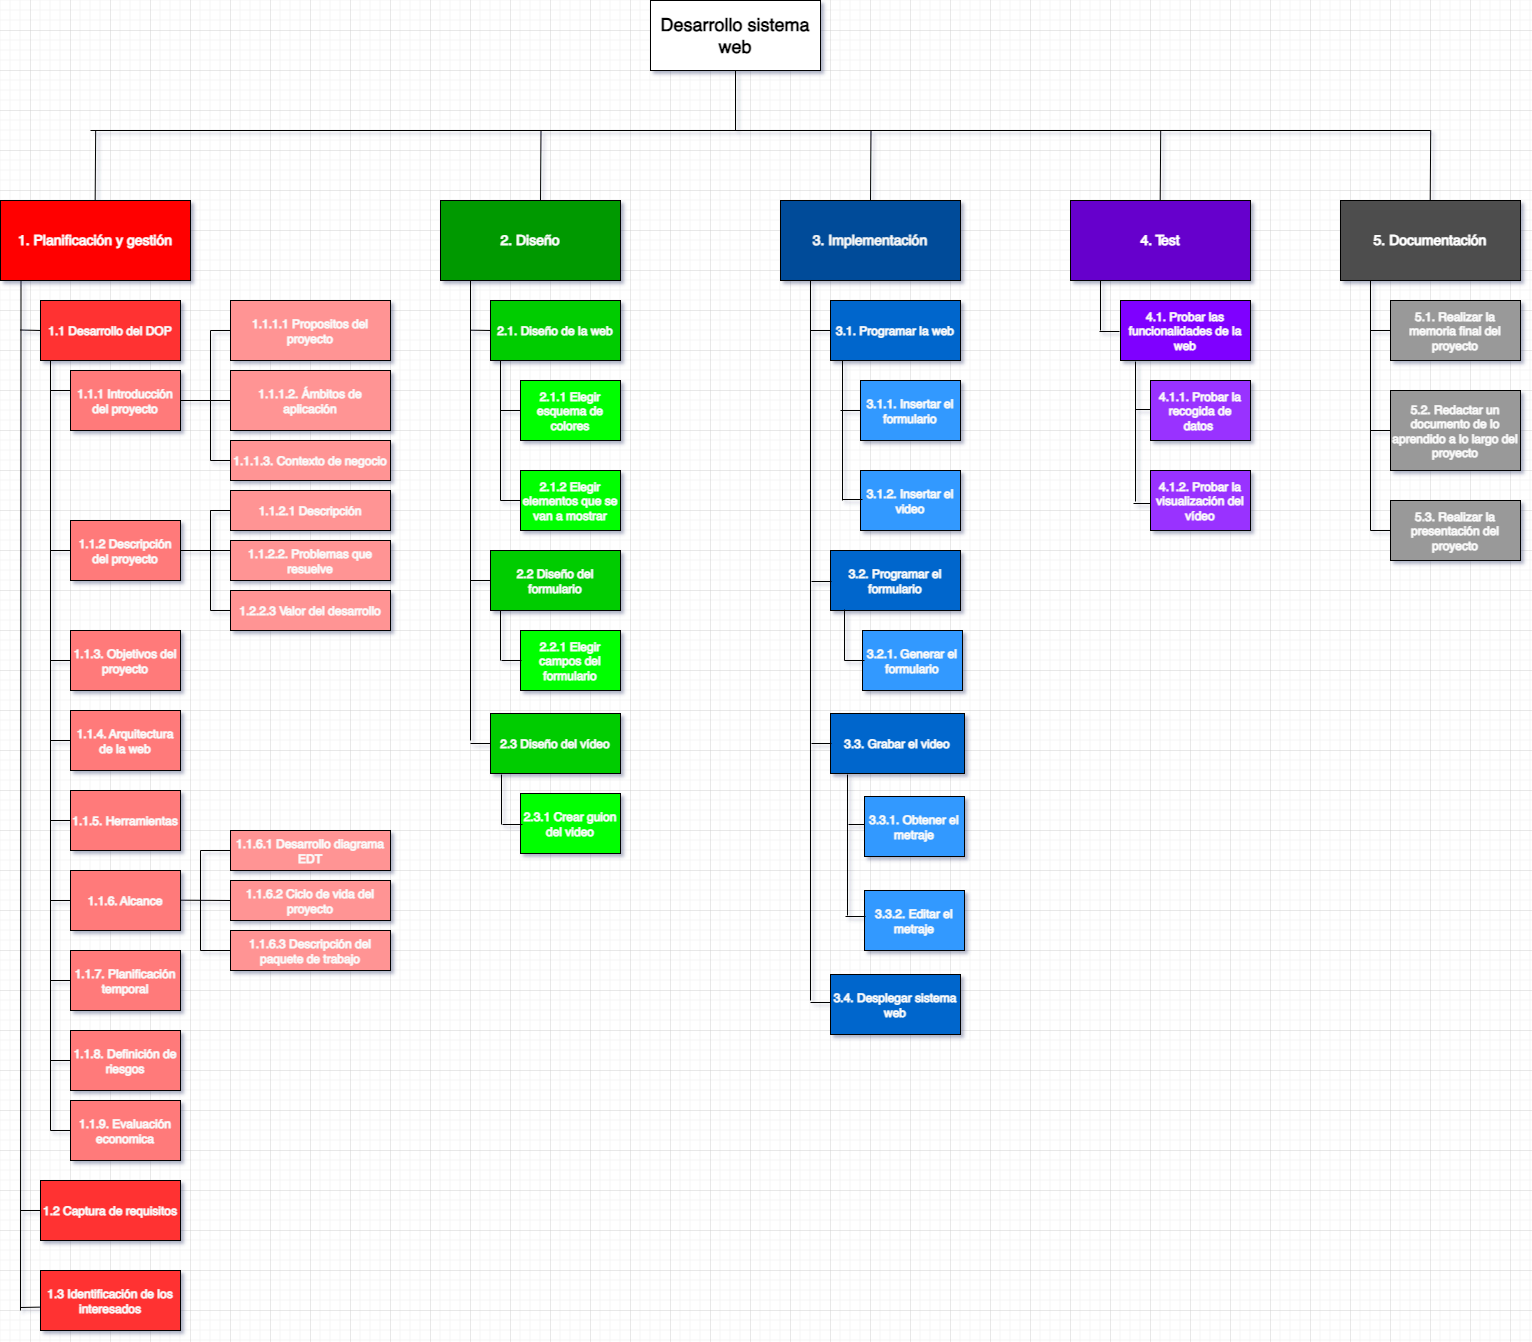
\includegraphics[width=1\textwidth]{./img/edt.png}
                \caption{EDT del proyecto}
            \end{figure}
            \clearpage
            \subsection{Planificación y Gestión}
                \begin{itemize}
                    \item Desarrollo del DOP (Duración: 43 días)
                    \begin{itemize}
                        \item Introducción del proyecto (Duración: 3 días)
                        \begin{itemize}
                            \item Describir en qué consiste el proyecto e identificar los objetivos del mismo
                        \end{itemize}
                        \item Descripción del proyecto (Duración: 3 días)
                        \begin{itemize}
                            \item Realizar una descripción del producto e identificar qué problemas soluciona
                        \end{itemize}
                        \item Objetivos del proyecto (Duración: 3 días)
                        \begin{itemize}
                            \item Establecer los objetivos que se quieren llevar a cabo en el proyecto
                        \end{itemize}
                        \item Arquitectura (Duración: 3 días)
                        \begin{itemize}
                            \item Identificar el tipo de estructura que va a tener el sistema y explicar cada una de sus partes
                        \end{itemize}
                        \item Herramientas (Duración: 3 días)
                        \begin{itemize}
                            \item Describir las herramientas que se van a utilizar y explicar el motivo de su elección
                        \end{itemize}
                        \item Alcance del proyecto (Duración: 13 días)
                        \begin{itemize}
                            \item Incluir el ciclo de vida del proyecto, diagrama de la estructura de descomposición del trabajo y una descripción de cada uno de los nodos
                        \end{itemize}
                        \item Planificación temporal (Duración: 6 días)
                        \begin{itemize}
                            \item Realizar una planificación temporal del proyecto usando un diagrama de Gantt
                        \end{itemize}
                        \item Riesgos (Duración: 3 días)
                        \begin{itemize}
                            \item Identificar los riesgos del proyecto y realizar una breve descripción de estos
                        \end{itemize}
                        \item Evaluación económica (Duración: 6 días)
                        \begin{itemize}
                            \item Hacer un análisis económico de los costes del proyecto
                        \end{itemize}
                    \end{itemize}
                    \item Captura de requisitos (Duración: 3 días)
                    \begin{itemize}
                        \item Identificar y describir los objetivos principales del proyecto
                    \end{itemize}
                    \item Identifiación de los interesados (Duración: 3 días)
                    \begin{itemize}
                        \item Identificar los interesados principales, su poder/interés en el proyecto y sus objetivos.
                    \end{itemize}
                \end{itemize}
                Duración total: 49 días
            \subsection{Diseño}
                \begin{itemize}
                    \item Diseño de la página web (Duración: 2 días)
                    \begin{itemize}
                        \item Hacer un boceto del sistema web
                    \end{itemize}
                    \item Diseño del video promocional (Duración: 3 día)
                    \begin{itemize}
                        \item Elegir la información que se va a transmitir en el video
                    \end{itemize}
                    \item Diseño del formulario de Google Forms (Duración: 1 días)
                    \begin{itemize}
                        \item Hacer un esquema del formulario
                    \end{itemize}
                \end{itemize}
                Duración total: 6 días
            \subsection{Implementación}
                \begin{itemize}
                    \item Programación de la página web (Duración: 2 días)
                    \begin{itemize}
                        \item Programar la página web
                    \end{itemize}
                    \item Grabación del video promocional (Duración: 6 días)
                    \begin{itemize}
                        \item Implementar el video en la página web
                    \end{itemize}
                    \item Implementación del formulario de Google Forms (Duración: 3 días)
                    \begin{itemize}
                        \item Implementar el formulario en la página web
                    \end{itemize}
                    \item Despliegue de la página web en Google Cloud (Duración: 6 días)
                    \begin{itemize}
                        \item Desplegar la página web en Google Cloud
                    \end{itemize}
                \end{itemize}
                Duración total: 17 días
            \subsection{Plan de pruebas}
                \begin{itemize}
                    \item Pruebas de la página web (Duración: 6 días)
                    \begin{itemize}
                        \item Realizar las pruebas de la página web
                    \end{itemize}
                    \item Pruebas del video promocional (Duración: 3 días)
                    \begin{itemize}
                        \item Realizar las correcta visualización del video en la página web
                    \end{itemize}
                    \item Pruebas del formulario de Google Forms (Duración: 3 días)
                    \begin{itemize}
                        \item Comprobar la correcta integración del formulario en la página web
                    \end{itemize}
                \end{itemize}
                Duración total: 6 días
            \subsection{Documentación}
                \begin{itemize}
                    \item Realizar la documentacion de la página web (Duración: 6 días)
                    \begin{itemize}
                        \item Describir el funcionamiento de la página web
                    \end{itemize}
                    \item Realizar la presentacion del proyecto (Duración: 6 días)
                    \begin{itemize}
                        \item Preparar la presentación del proyecto
                    \end{itemize}
                \end{itemize}
                Duración total: 12 días
            \vfill
        \begin{center}
            Duración total del proyecto: 90 días
        \end{center}
    \chapter{Planificación temporal}
        \paragraph*{}{
            Para la planificación temporal del proyecto hemos decidido utilizar un diagrama de Gantt. En este diagrama se muestra la duración de cada tarea y el esfuerzo que se le ha dedicado. Además, se ha incluido una tabla con la duración y el esfuerzo de cada tarea.
        }
        \begin{center}
            \begin{longtable}{|p{7cm}|p{3cm}|p{3cm}|}
                \hline
                \textbf{Fase/Tarea} & \textbf{Esfuerzo (persona-tiempo)} & \textbf{Duración (tiempo)}\\
                \hline
                \hline
                \textbf{1. Planificación y Gestión} &  &  \\
                \hline
                1.1 Desarrollo del DOP &  & \\
                \hline
                1.1.1 Introduccion del proyecto &  & \\
                \hline
                1.1.1.1 Proposito del proyecto & 1 persona-dia & 1 día\\
                \hline
                1.1.1.2 Ambitos de aplicacion & 1 persona-dia & 1 día\\
                \hline
                1.1.1.3 Contexto de negocio & 1 persona-dia & 1 día\\
                \hline
                1.1.2 Descripcion del proyecto &  & \\
                \hline
                1.1.2.1 Descripción & 1 persona-dia & 1 día\\
                \hline
                1.1.2.2 Problemas que resuelve & 1 persona-dia & 1 día\\
                \hline
                1.1.2.3 Valor del desarrollo & 1 persona-dia & 1 día\\
                \hline
                1.1.3 Objetivos del proyecto & 3 persona-dia & 3 día\\
                \hline
                1.1.4 Arquitectura & 3 persona-dia & 3 día\\
                \hline
                1.1.5 Herramientas & 3 persona-dia & 3 día\\
                \hline
                1.1.6 Alcance del proyecto &  & \\
                \hline
                1.1.6.1 Planificacion temporal & 6 persona-dia & 6 día\\
                \hline
                1.1.6.2 Ciclo de vida & 1 persona-dia & 1 día\\
                \hline
                1.1.6.3 Descripción de los paquetes de trabajo & 12 persona-dia & 6 día\\
                \hline
                1.1.7 Planificacion temporal & 12 persona-dia & 6 día\\
                \hline
                1.1.8 Riesgos & 3 persona-dia & 3 día\\
                \hline
                1.1.9 Evaluacion economica & 6 persona-dia & 6 día\\
                \hline
                1.2 Captura de requisitos & 3 persona-dia & 3 día\\
                \hline
                1.3 Identificacion de los interesados & 3 persona-dia & 3 día\\
                \hline
                \textbf{2. Diseño} &  & \\
                \hline
                2.1 Diseño de la web &  & \\
                \hline
                2.1.1 Elegir esquema de colores & 6 persona-dia & 1 día\\
                \hline
                2.1.2 Elegir elementos que se van a mostrar & 6 persona-dia & 1 día\\
                \hline
                2.2 Diseño del formulario\\
                \hline
                2.2.1 Elegir campos del formulario & 6 persona-dia & 1 día\\
                \hline
                2.3 Diseño del video & & \\
                \hline
                2.3.1 Crear guion del video & 18 persona-dia & 3 día\\
                \hline
                \textbf{3. Implementación} &  & \\
                \hline
                3.1 Programación la web &  & \\
                \hline
                3.1.1 Insertar el formulario & 1 persona-dia & 1 día\\
                \hline
                3.1.2 Insertar el video & 1 persona-dia & 1 día\\
                \hline
                3.2 Programación del formulario\\
                \hline
                3.2.1 Generar el formulario & 3 persona-dia & 3 día\\
                \hline
                3.3 Grabar el video\\
                \hline
                3.3.1 Obtener el metraje & 3 persona-dia & 3 día\\
                \hline
                3.3.2 Editar el metraje & 18 persona-dia & 6 día\\
                \hline
                3.4 Despliegue de la web en Google Cloud & 6 persona-dia & 6 día\\
                \hline
                \textbf{4. Plan de pruebas} &  & \\
                \hline
                4.1 Pruebas de la web & & \\
                \hline
                4.1.1 Pruebas la recogida de datos & 18 persona-dia & 3 día\\
                \hline
                4.2 Pruebas del video & 18 persona-dia & 3 día\\
                \hline
                \textbf{5. Documentación} &  & \\
                \hline
                5.1 Documentación de la web & 36 persona-dia & 6 día\\
                \hline
                5.2 Presentación del proyecto & 36 persona-dia & 6 día\\
                \hline
                \hline
                \textbf{Total} &  & 90 días\\
                \hline
                \caption{Planificacion temporal}
            \end{longtable}
            \begin{figure}[H]
                \centering
                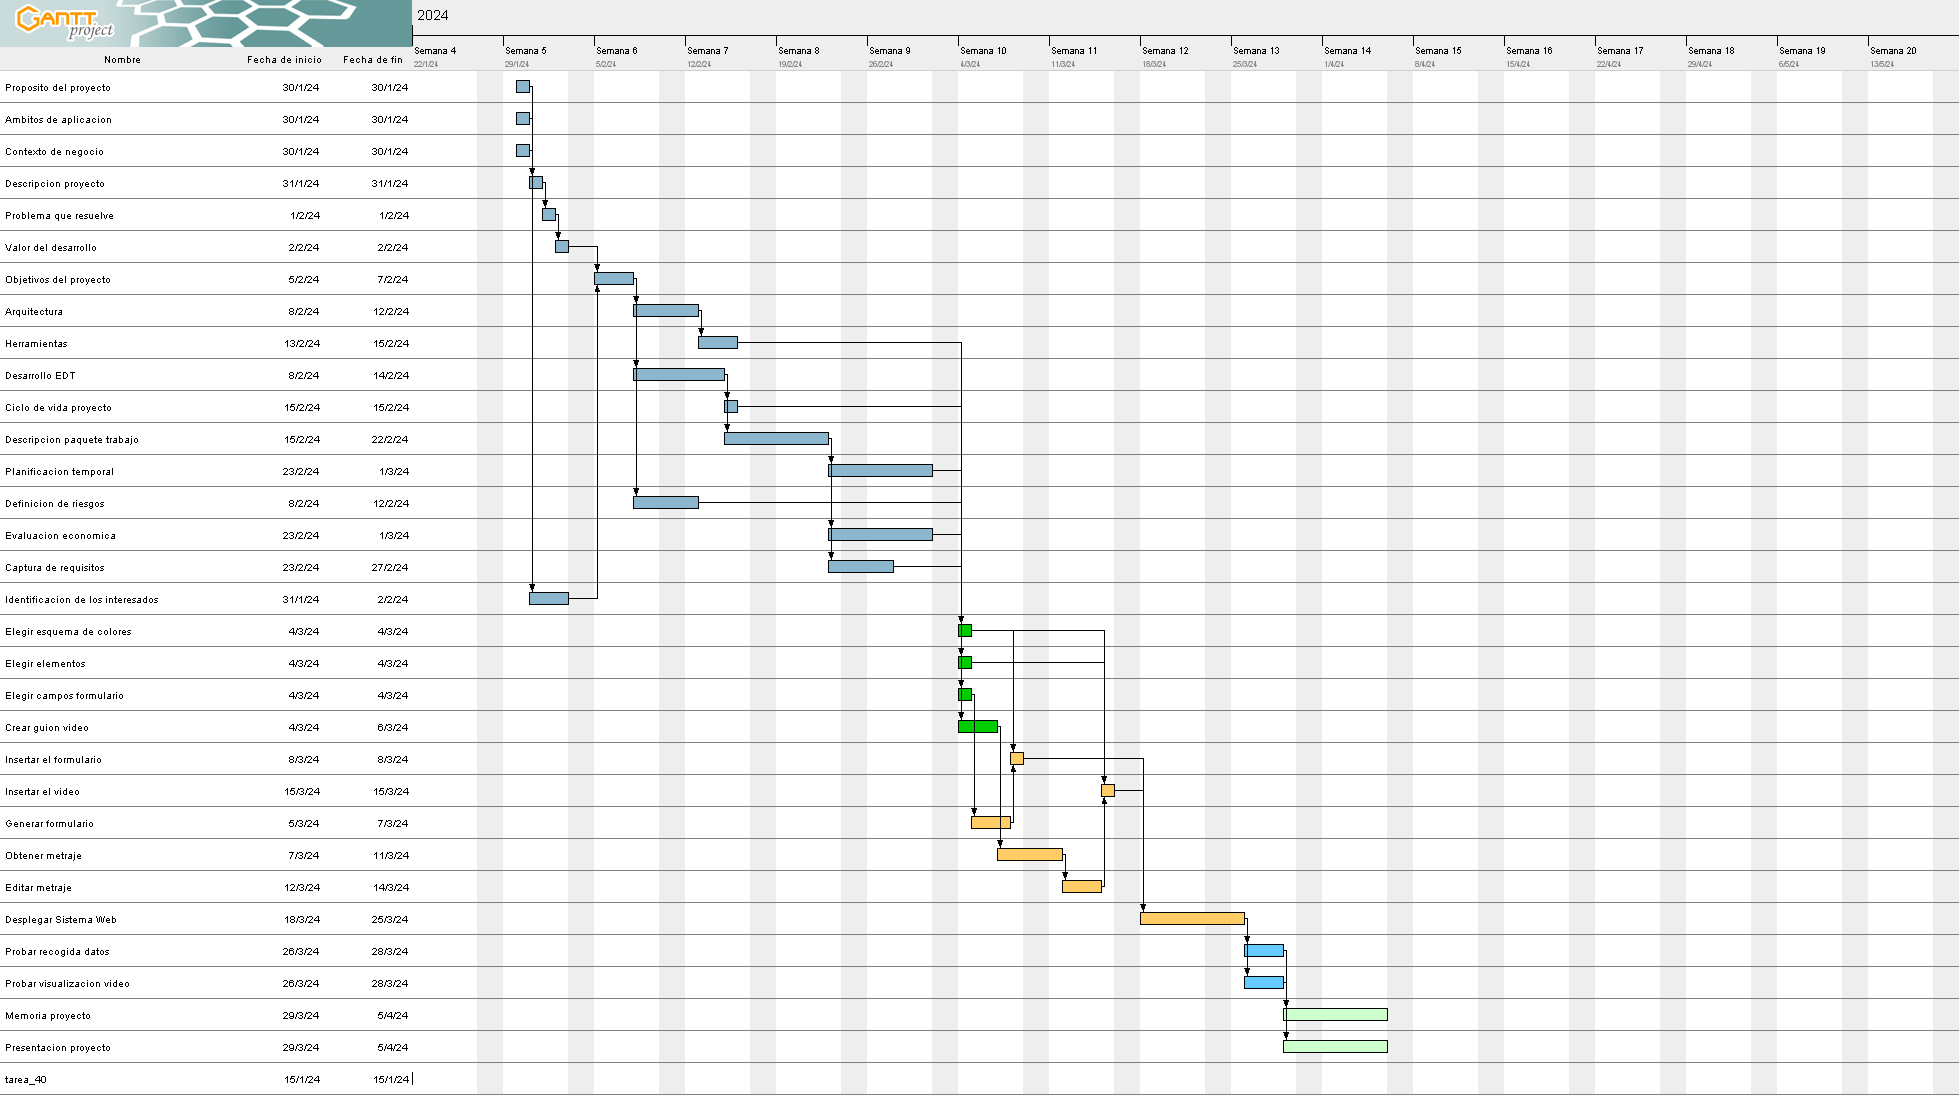
\includegraphics[width=1\textwidth]{./img/gantt.png}
                \caption{Diagrama de Gantt}
            \end{figure}
        \end{center}
        \paragraph*{}{
            Las holguras de las tareas pueden ser visto en el Anexo \ref{roy}
        }
        \paragraph*{Camino critico general: }{1.1.1.1/1.1.1.2/1.1.1.3 - 1.1.2.1 - 1.1.2.2 - 1.1.2.3 / 1.3 - 1.1.3 - 1.1.6.1 - 1.1.6.3 - 1.1.7 / 1.1.9 - 2.3.1 - 3.3.1 - 3.3.2 - 3.1.1 / 3.1.2 - 3.4 - 4.1 / 4.2 - 5.1 / 5.2}
    \chapter{Riesgos}
        \paragraph*{}{
            La gestion de riesgos es un proceso que permite identificar, evaluar y priorizar los riesgos del proyecto. A continuación, se presentan los riesgos identificados en el proyecto, junto con su prevención y plan de contingencia.
        }
        \begin{center}
            \begin{longtable}{|p{6cm}|p{6cm}|}
                \hline
                \textbf{Descripción} & Que un agente externo mediante una vulnerabilidad de seguridad pueda realizar acciones no autorizadas en la página web.\\
                \hline
                \textbf{Prevención} & Realizar pruebas de seguridad en la página web.\\
                \hline
                \textbf{Plan de contingencia} & Parchear la vulnerabilidad y realizar una auditoría de seguridad en la página web.\\
                \hline
                \textbf{Probabilidad} & Media\\
                \hline
                \textbf{Impacto} & Muy alto\\
                \hline
                \caption{Vulnerabilidades de seguridad}
            \end{longtable}
        \end{center}
        \begin{center}
            \begin{longtable}{|p{6cm}|p{6cm}|}
                \hline
                \textbf{Descripción} & Perder toda o parte de la información almacenada en Google Forms.\\
                \hline
                \textbf{Prevención} & Guardar copias de seguridad de la información en un lugar seguro.\\
                \hline
                \textbf{Plan de contingencia} & Utilizar las copias de seguridad para recuperar la información perdida.\\
                \hline
                \textbf{Probabilidad} & Baja\\
                \hline
                \textbf{Impacto} & Muy alto\\
                \hline
                \caption{Perdida de información}
            \end{longtable}
        \end{center}
        \begin{center}
            \begin{longtable}{|p{6cm}|p{6cm}|}
                \hline
                \textbf{Descripción} & La información almacenada en Google Forms es accedida por un tercero.\\
                \hline
                \textbf{Prevención} & Cifrar la conexion con la web y usar contraseña seguras con 2FA en la cuenta de Google.\\
                \hline
                \textbf{Plan de contingencia} & Generar nuevos certificados para la web y nueva contraseña para la cuenta de Google.\\
                \hline
                \textbf{Probabilidad} & Baja\\
                \hline
                \textbf{Impacto} & Medio\\
                \hline
                \caption{Seguridad de datos}
            \end{longtable}
        \end{center}
        \clearpage
        \begin{center}
            \begin{longtable}{|p{6cm}|p{6cm}|}
                \hline
                \textbf{Descripción} & Los navegadores no muestra parte o la totalidad de la página web correctamente.\\
                \hline
                \textbf{Prevención} & Probar de forma periodica la página web en los navegadores más utilizados.\\
                \hline
                \textbf{Plan de contingencia} & Modificar la página web para que sea compatible con los navegadores actuales en el menor tiempo posible.\\
                \hline
                \textbf{Probabilidad} & Muy baja\\
                \hline
                \textbf{Impacto} & Alto\\
                \hline
                \caption{Compatibilidad de navegadores}
            \end{longtable}
        \end{center}
        \begin{center}
            \begin{longtable}{|p{6cm}|p{6cm}|}
                \hline
                \textbf{Descripción} & La pagina web sufre caidas debido a la gran cantidad de usuarios que acceden a ella o a ataques de denegación de servicio.\\
                \hline
                \textbf{Prevención} & Realizar pruebas de carga en la página web.\\
                \hline
                \textbf{Plan de contingencia} & Aumentar la capacidad de la página web mediante la creación de más contenedores cuando sea necesario (escalado horizontal).\\
                \hline
                \textbf{Probabilidad} & Alta\\
                \hline
                \textbf{Impacto} & Alto\\
                \hline
                \caption{Problemas de escalabilidad}
            \end{longtable}
        \end{center}
        \begin{center}
            \begin{longtable}{|p{6cm}|p{6cm}|}
                \hline
                \textbf{Descripción} & La pagina tarda en cargar debido a el peso de los elementos multimedia.\\
                \hline
                \textbf{Prevención} & Realizar pruebas de carga en la página web.\\
                \hline
                \textbf{Plan de contingencia} & Cambiar la codificación de los elementos multimedia para que pesen menos.\\
                \hline
                \textbf{Probabilidad} & Media\\
                \hline
                \textbf{Impacto} & Muy bajo\\
                \hline
                \caption{Elementos pesados}
            \end{longtable}
        \end{center}
    \chapter{Evaluación económica}
        \paragraph*{}
        {
            En todo proyecto es necesario realizar una evaluación económica para saber la viabilidad del mismo.\\

            En cuanto a los costes de personal, se ha estimado un coste de \textbf{20€/hora} por persona.
            Sabiendo que somos 6 personas trabajando en el proyecto y con un esfuerzo total 90 dias con 3 horas de trabajo o 270 horas, se ha estimado un coste total de \textbf{5400€}.
            A esto habria que sumarle los costes de la seguridad social, que se estiman en un 30\% del coste total de personal, es decir, \textbf{1620€}.
            Por lo tanto, el coste total de personal sería de \textbf{7020€}.\\

            En lo referente al material, al tratarse de un proyecto de desarrollo web, debemos dividirlo en dos partes: el hardware y el software.\\
            \begin{itemize}
                \item En cuanto al hardware, tenemos que tener en cuenta que se ha utilizado un ordenador por persona, un dispositivo movil, una camara de video un microfono y un servidor.
                \begin{itemize}
                    \item Cada ordenador tiene un coste aproximado de \textbf{1000€} y tienen una vida media de 5 años por lo que la amortización anual sería de \textbf{200€}. Dado que el uso del proyecto es de 3 meses y el porcentaje de uso es del 33\%, el coste total sería de \textbf{16,5€} por cabeza, es decir, \textbf{99€} en total.
                    \item El móvil tiene un coste aproximado de \textbf{500€} y tiene una vida media de 5 años por lo que la amortización anual sería de \textbf{100€}. Dado que el uso del proyecto es de 3 meses y el porcentaje de uso es del 33\%, el coste total sería de \textbf{8,25€} por cabeza, es decir, \textbf{49.5€} en total.
                    \item La camara de video tiene un coste aproximado de \textbf{500€} y tiene una vida media de 5 años por lo que la amortización anual sería de \textbf{100€}. Dado que el uso del proyecto es de 3 meses y el porcentaje de uso es del 5\%, el coste total sería de \textbf{1,25€}
                    \item El microfono tiene un coste aproximado de \textbf{100€} y tiene una vida media de 5 años por lo que la amortización anual sería de \textbf{20€}. Dado que el uso del proyecto es de 3 meses y el porcentaje de uso es del 5\%, el coste total sería de \textbf{0,25€}
                    \item El servidor tiene un coste aproximado de \textbf{144€} anuales. Dado que el uso del proyecto es de 3 meses y el porcentaje de uso es del 100\%, el coste total sería de \textbf{36€}.
                    \item En total, el coste de hardware sería de \textbf{186€}.
                \end{itemize}
                \item En cuanto al software, el equipo esta concienciado con el software libre y por ello se ha utilizado software libre en todo el proyecto. Por lo tanto, el coste de software sería de \textbf{0€}.
                \item En lo que refiere a costes indirectos como la luz y el acceso a internet, se ha estimado un coste de \textbf{20€} por persona. Un total de \textbf{120€}.
            \end{itemize}
            Por lo tanto, el coste total del proyecto sería de \textbf{7326€}.
        }
    \chapter{Anexo} %TODO
        \section{Paquetes de trabajo}
            \begin{center}
                \begin{longtable}{|p{6cm}|p{6cm}|}
                    \hline
                    \textbf{Paquete de trabajo:} & Propósitos del proyecto (1.1.1.1)\\
                    \hline
                    \textbf{Responsable} & Pablo Leclercq\\
                    \hline
                    \textbf{Esfuerzo} & 1 día\\
                    \hline
                    \textbf{Descripción} & Explicar los propósitos de este proyecto\\
                    \hline
                    \textbf{Entradas} & Hemos utilizado la plantilla y nos hemos basado en el ejemplo facilitado\\
                    \hline
                    \textbf{Salidas/Entregables} & Ninguna\\
                    \hline
                    \textbf{Hitos} & No se ha conseguido ningún hito\\
                    \hline
                    \textbf{Recursos necesarios} & Solo se ha necesitado un analista y hemos utilizado libreoffice y latex para hacer esta parte de la documentación\\
                    \hline
                    \textbf{Precedencias} & Ninguna\\
                    \hline
                    \caption{Propósitos del proyecto}
                \end{longtable}
                \begin{longtable}{|p{6cm}|p{6cm}|}
                    \hline
                    \textbf{Paquete de trabajo:} & Ámbitos de aplicación (1.1.1.2)\\
                    \hline
                    \textbf{Responsable} & Pablo Leclercq\\
                    \hline
                    \textbf{Esfuerzo} & 1 día\\
                    \hline
                    \textbf{Descripción} & Indicar con qué otros proyectos está relacionado este proyecto y en que tipos de dispositivos va a funcionar\\
                    \hline
                    \textbf{Entradas} & Hemos utilizado la plantilla y nos hemos basado en el ejemplo facilitado\\
                    \hline
                    \textbf{Salidas/Entregables} & Ninguna\\
                    \hline
                    \textbf{Hitos} & No se ha conseguido ningún hito\\
                    \hline
                    \textbf{Recursos necesarios} & Solo se ha necesitado un analista y hemos utilizado libreoffice y latex para hacer esta parte de la documentación\\
                    \hline
                    \textbf{Precedencias} & Ninguna\\
                    \hline
                    \caption{Ámbitos de aplicación}
                \end{longtable}
                \clearpage
                \begin{longtable}{|p{6cm}|p{6cm}|}
                    \hline
                    \textbf{Paquete de trabajo:} & Contexto de negocio (1.1.1.3)\\
                    \hline
                    \textbf{Responsable} & Pablo Leclercq\\
                    \hline
                    \textbf{Esfuerzo} & 1 día\\
                    \hline
                    \textbf{Descripción} & Definición del contexto de negocio del proyecto, por ejemplo, el área y el mercado en el que se va a utilizar, los usuarios que lo van a usar… Además de una definición de los términos necesarios para entender el proyecto \\
                    \hline
                    \textbf{Entradas} & Hemos utilizado la plantilla y nos hemos basado en el ejemplo facilitado\\
                    \hline
                    \textbf{Salidas/Entregables} & Ninguna\\
                    \hline
                    \textbf{Hitos} & No se ha conseguido ningún hito\\
                    \hline
                    \textbf{Recursos necesarios} & Solo se ha necesitado un analista y hemos utilizado libreoffice y latex para hacer esta parte de la documentación\\
                    \hline
                    \textbf{Precedencias} & Ninguna\\
                    \hline
                    \caption{Contexto de negocio}
                \end{longtable}
                \begin{longtable}{|p{6cm}|p{6cm}|}
                    \hline
                    \textbf{Paquete de trabajo:} & Descripción (1.1.2.1)\\
                    \hline
                    \textbf{Responsable} & Pablo Leclercq\\
                    \hline
                    \textbf{Esfuerzo} & 1 día\\
                    \hline
                    \textbf{Descripción} & Definición del contexto de negocio del proyecto, por ejemplo, el área y el mercado en el que se va a utilizar, los usuarios que lo van a usar… Además de una definición de los términos necesarios para entender el proyecto \\
                    \hline
                    \textbf{Entradas} & Hemos utilizado la plantilla y nos hemos basado en el ejemplo facilitado\\
                    \hline
                    \textbf{Salidas/Entregables} & Ninguna\\
                    \hline
                    \textbf{Hitos} & No se ha conseguido ningún hito\\
                    \hline
                    \textbf{Recursos necesarios} & Solo se ha necesitado un analista y hemos utilizado libreoffice y latex para hacer esta parte de la documentación\\
                    \hline
                    \textbf{Precedencias} & 1.1.1.1 Proposito del proyecto,
                                            1.1.1.2 Ámbitos de aplicación,
                                            1.1.1.3 Contexto de negocio\\
                    \hline
                    \caption{Descripción}
                \end{longtable}
                \clearpage
                \begin{longtable}{|p{6cm}|p{6cm}|}
                    \hline
                    \textbf{Paquete de trabajo:} & Problemas que resuelve (1.1.2.2)\\
                    \hline
                    \textbf{Responsable} & Pablo Leclercq\\
                    \hline
                    \textbf{Esfuerzo} & 1 día\\
                    \hline
                    \textbf{Descripción} & Explicar los problemas que resuelve este proyecto\\
                    \hline
                    \textbf{Entradas} & Hemos utilizado la plantilla y nos hemos basado en el ejemplo facilitado\\
                    \hline
                    \textbf{Salidas/Entregables} & Ninguna\\
                    \hline
                    \textbf{Hitos} & No se ha conseguido ningún hito\\
                    \hline
                    \textbf{Recursos necesarios} & Solo se ha necesitado un analista y hemos utilizado libreoffice y latex para hacer esta parte de la documentación\\
                    \hline
                    \textbf{Precedencias} & 1.1.2.1 Descripción\\
                    \hline
                    \caption{Problemas que resuelve}
                \end{longtable}
                \begin{longtable}{|p{6cm}|p{6cm}|}
                    \hline
                    \textbf{Paquete de trabajo:} & Valor del desarrollo (1.1.2.3)\\
                    \hline
                    \textbf{Responsable} & Pablo Leclercq\\
                    \hline
                    \textbf{Esfuerzo} & 1 día\\
                    \hline
                    \textbf{Descripción} & Explicar el valor que tiene desarrollar un proyecto de este estilo\\
                    \hline
                    \textbf{Entradas} & Hemos utilizado la plantilla y nos hemos basado en el ejemplo facilitado\\
                    \hline
                    \textbf{Salidas/Entregables} & Ninguna\\
                    \hline
                    \textbf{Hitos} & No se ha conseguido ningún hito\\
                    \hline
                    \textbf{Recursos necesarios} & Solo se ha necesitado un analista y hemos utilizado libreoffice y latex para hacer esta parte de la documentación\\
                    \hline
                    \textbf{Precedencias} & 1.1.2.2 Problemas que resuelve\\
                    \hline
                    \caption{Valor del desarrollo}
                \end{longtable}
                \clearpage
                \begin{longtable}{|p{6cm}|p{6cm}|}
                    \hline
                    \textbf{Paquete de trabajo:} & Objetivos del proyecto (1.1.3)\\
                    \hline
                    \textbf{Responsable} & Pablo Leclercq\\
                    \hline
                    \textbf{Esfuerzo} & 1 día\\
                    \hline
                    \textbf{Descripción} & Establecer los objetivos que se quieren llevar a cabo en el proyecto teniendo en cuenta cinco niveles (específico, medible, alcanzable, relevante y temporal)\\
                    \hline
                    \textbf{Entradas} & Hemos utilizado la plantilla y nos hemos basado en el ejemplo facilitado\\
                    \hline
                    \textbf{Salidas/Entregables} & Ninguna\\
                    \hline
                    \textbf{Hitos} & No se ha conseguido ningún hito\\
                    \hline
                    \textbf{Recursos necesarios} & Solo se ha necesitado un analista y hemos utilizado libreoffice y latex para hacer esta parte de la documentación\\
                    \hline
                    \textbf{Precedencias} & 1.1.2.3 Valor del desarrollo,
                                            1.3 Identificación de los interesados\\
                    \hline
                    \caption{Objetivos del proyecto}
                \end{longtable}
                \begin{longtable}{|p{6cm}|p{6cm}|}
                    \hline
                    \textbf{Paquete de trabajo:} & Arquitectura (1.1.4)\\
                    \hline
                    \textbf{Responsable} & Ander Gorocica\\
                    \hline
                    \textbf{Esfuerzo} & 3 días\\
                    \hline
                    \textbf{Descripción} & Explicar los componentes de la arquitectura de la página web y el funcionamiento de esta arquitectura acompañado de un esquema.\\
                    \hline
                    \textbf{Entradas} & Hemos utilizado la plantilla y nos hemos basado en el ejemplo facilitado\\
                    \hline
                    \textbf{Salidas/Entregables} & Ninguna\\
                    \hline
                    \textbf{Hitos} & No se ha conseguido ningún hito\\
                    \hline
                    \textbf{Recursos necesarios} & Solo se ha necesitado un programador y hemos utilizado libreoffice y latex para hacer esta parte de la documentación\\
                    \hline
                    \textbf{Precedencias} & 1.1.3 Objetivos del proyecto\\
                    \hline
                    \caption{Arquitectura}
                \end{longtable}
                \clearpage
                \begin{longtable}{|p{6cm}|p{6cm}|}
                    \hline
                    \textbf{Paquete de trabajo:} & Herramientas (1.1.5)\\
                    \hline
                    \textbf{Responsable} & Asier Larrazabal\\
                    \hline
                    \textbf{Esfuerzo} & 3 días\\
                    \hline
                    \textbf{Descripción} & Explicar todas las aplicaciones y herramientas que usaremos a la hora de realizar este proyecto, realizando una breve descripción de para qué usamos cada una.\\
                    \hline
                    \textbf{Entradas} & Hemos utilizado la plantilla y nos hemos basado en el ejemplo facilitado\\
                    \hline
                    \textbf{Salidas/Entregables} & Ninguna\\
                    \hline
                    \textbf{Hitos} & No se ha conseguido ningún hito\\
                    \hline
                    \textbf{Recursos necesarios} & Solo se ha necesitado un programador y hemos utilizado libreoffice y latex para hacer esta parte de la documentación\\
                    \hline
                    \textbf{Precedencias} & 1.1.4 Arquitectura\\
                    \hline
                    \caption{Herramientas}
                \end{longtable}
                \begin{longtable}{|p{6cm}|p{6cm}|}
                    \hline
                    \textbf{Paquete de trabajo:} & Desarrollo del diagrama del EDT (1.1.6.1)\\
                    \hline
                    \textbf{Responsable} & Ander Gorocica\\
                    \hline
                    \textbf{Esfuerzo} & 6 días\\
                    \hline
                    \textbf{Descripción} & Elaboración del díagrama del EDT que representa todas las tareas que componen el proyecto. En este esquema se muestra en forma de árbol los nombres de todas las tareas y subtareas que nos componen.\\
                    \hline
                    \textbf{Entradas} & Hemos utilizado la plantilla y nos hemos basado en el ejemplo facilitado\\
                    \hline
                    \textbf{Salidas/Entregables} & Ninguna\\
                    \hline
                    \textbf{Hitos} & No se ha conseguido ningún hito\\
                    \hline
                    \textbf{Recursos necesarios} & Solo se ha necesitado un analista y hemos utilizado libreoffice y latex para hacer esta parte de la documentación\\
                    \hline
                    \textbf{Precedencias} & 1.1.3 Objetivos del proyecto\\
                    \hline
                    \caption{Desarrollo del diagrama del EDT}
                \end{longtable}
                \clearpage
                \begin{longtable}{|p{6cm}|p{6cm}|}
                    \hline
                    \textbf{Paquete de trabajo:} & Ciclo de vida del proyecto (1.1.6.2)\\
                    \hline
                    \textbf{Responsable} & Xabier Badiola\\
                    \hline
                    \textbf{Esfuerzo} & 1 días\\
                    \hline
                    \textbf{Descripción} & Descripción del ciclo de vida del proyecto acompañado de un esquema.\\
                    \hline
                    \textbf{Entradas} & Hemos utilizado la plantilla y nos hemos basado en el ejemplo facilitado\\
                    \hline
                    \textbf{Salidas/Entregables} & Ninguna\\
                    \hline
                    \textbf{Hitos} & No se ha conseguido ningún hito\\
                    \hline
                    \textbf{Recursos necesarios} & Se han necesitado un analista y hemos utilizado libreoffice y latex para hacer esta parte de la documentación\\
                    \hline
                    \textbf{Precedencias} & 1.1.6.1 Desarrollo del diagrama del EDT\\
                    \hline
                    \caption{Ciclo de vida del proyecto}
                \end{longtable}
                \begin{longtable}{|p{6cm}|p{6cm}|}
                    \hline
                    \textbf{Paquete de trabajo:} & Descripción del paquete de trabajo (1.1.6.3)\\
                    \hline
                    \textbf{Responsable} & Xabier Badiola y Ander Gorocica\\
                    \hline
                    \textbf{Esfuerzo} & 6 días\\
                    \hline
                    \textbf{Descripción} & Descripción breve de todas las tareas que componen el díagrama del EDT y la descripción detallada de todos los nodos hoja del díagrama del árbol.\\
                    \hline
                    \textbf{Entradas} & Hemos utilizado la plantilla y nos hemos basado en el ejemplo facilitado\\
                    \hline
                    \textbf{Salidas/Entregables} & Ninguna\\
                    \hline
                    \textbf{Hitos} & M1: Fin de la primera parte del DOP\\
                    \hline
                    \textbf{Recursos necesarios} & Se han necesitado tres analistas y hemos utilizado libreoffice, latex y gantt project para hacer esta parte de la documentación\\
                    \hline
                    \textbf{Precedencias} & 1.1.6.1 Desarrollo del diagrama del EDT\\
                    \hline
                    \caption{Descripción del paquete de trabajo}
                \end{longtable}
                \clearpage
                \begin{longtable}{|p{6cm}|p{6cm}|}
                    \hline
                    \textbf{Paquete de trabajo:} & Planificación temporal (1.1.7)\\
                    \hline
                    \textbf{Responsable} & Pablo Leclercq y Ander Gorocica\\
                    \hline
                    \textbf{Esfuerzo} & 6 días\\
                    \hline
                    \textbf{Descripción} & Realización de una planificación temporal utilizando CPM, ROY o la técnica de precedencias, el díagrama de Gantt y una tabla que recoge todas las fases y tareas con el esfuerzo y la duración de cada una.\\
                    \hline
                    \textbf{Entradas} & Hemos utilizado la plantilla y nos hemos basado en el ejemplo facilitado\\
                    \hline
                    \textbf{Salidas/Entregables} & Ninguna\\
                    \hline
                    \textbf{Hitos} & No se ha conseguido ningún hito\\
                    \hline
                    \textbf{Recursos necesarios} & Se necesitan dos analistas y hemos utilizado libreoffice y latex para hacer esta parte de la documentación\\
                    \hline
                    \textbf{Precedencias} & 1.1.6.3 Descripción del paquete de trabajo\\
                    \hline
                    \caption{Planificación temporal}
                \end{longtable}
                \begin{longtable}{|p{6cm}|p{6cm}|}
                    \hline
                    \textbf{Paquete de trabajo:} & Riesgos (1.1.8)\\
                    \hline
                    \textbf{Responsable} & Xabier Gabiña\\
                    \hline
                    \textbf{Esfuerzo} & 3 días\\
                    \hline
                    \textbf{Descripción} & Descripción de todos los riesgos que puede tener el desarrollo del proyecto\\
                    \hline
                    \textbf{Entradas} & Hemos utilizado la plantilla y nos hemos basado en el ejemplo facilitado\\
                    \hline
                    \textbf{Salidas/Entregables} & Ninguna\\
                    \hline
                    \textbf{Hitos} & No se ha conseguido ningún hito\\
                    \hline
                    \textbf{Recursos necesarios} & Se han necesitado un analista y hemos utilizado libreoffice y latex para hacer esta parte de la documentación\\
                    \hline
                    \textbf{Precedencias} & 1.1.3 Objetivos del proyecto\\
                    \hline
                    \caption{Riesgos}
                \end{longtable}
                \clearpage
                \begin{longtable}{|p{6cm}|p{6cm}|}
                    \hline
                    \textbf{Paquete de trabajo:} & Evaluación económica (1.1.9)\\
                    \hline
                    \textbf{Responsable} & Xabier Gabiña\\
                    \hline
                    \textbf{Esfuerzo} & 6 días\\
                    \hline
                    \textbf{Descripción} & Estimación de los gastos que supone el desarrollo del proyecto a nivel de personal, hardware y software y costes indirectos.\\
                    \hline
                    \textbf{Entradas} & Hemos utilizado la plantilla y nos hemos basado en el ejemplo facilitado\\
                    \hline
                    \textbf{Salidas/Entregables} & Documento DOP\\
                    \hline
                    \textbf{Hitos} & M2: Fin del Desarrollo del DOP\\
                    \hline
                    \textbf{Recursos necesarios} & Se han necesitado un analista y hemos utilizado libreoffice y latex para hacer esta parte de la documentación\\
                    \hline
                    \textbf{Precedencias} & 1.1.6.3 Descripción del paquete de trabajo\\
                    \hline
                    \caption{Evaluación económica}
                \end{longtable}
                \begin{longtable}{|p{6cm}|p{6cm}|}
                    \hline
                    \textbf{Paquete de trabajo:} & Captura de requisitos (1.2)\\
                    \hline
                    \textbf{Responsable} & Xabier Gabiña\\
                    \hline
                    \textbf{Esfuerzo} & 3 días\\
                    \hline
                    \textbf{Descripción} & Identificación y descripción de los requisitos del proyecto.\\
                    \hline
                    \textbf{Entradas} & Hemos utilizado la plantilla\\
                    \hline
                    \textbf{Salidas/Entregables} & Documento de captura de requisitos\\
                    \hline
                    \textbf{Hitos} & No se ha conseguido ningún hito\\
                    \hline
                    \textbf{Recursos necesarios} & Solo se ha necesitado un analista y hemos utilizado libreoffice y latex para hacer esta parte de la documentación\\
                    \hline
                    \textbf{Precedencias} & Ninguna\\
                    \hline
                    \caption{Captura de requisitos}
                \end{longtable}
                \clearpage
                \begin{longtable}{|p{6cm}|p{6cm}|}
                    \hline
                    \textbf{Paquete de trabajo:} & Identificación de los interesados (1.3)\\
                    \hline
                    \textbf{Responsable} & Xabier Gabiña\\
                    \hline
                    \textbf{Esfuerzo} & 3 días\\
                    \hline
                    \textbf{Descripción} & Identificación de los interesados y descripción de los objetivos que tienen respecto al proyecto, la influencia que tienen, como y cuando se realizan reuniones y se solucionan los problemas que surjan con el interesado.\\
                    \hline
                    \textbf{Entradas} & Hemos utilizado la plantilla\\
                    \hline
                    \textbf{Salidas/Entregables} & Documento de identificación de los interesados\\
                    \hline
                    \textbf{Hitos} & No se ha conseguido ningún hito\\
                    \hline
                    \textbf{Recursos necesarios} & Solo se ha necesitado un analista y hemos utilizado libreoffice y latex para hacer esta parte de la documentación\\
                    \hline
                    \textbf{Precedencias} & Ninguna\\
                    \hline
                    \caption{Identificación de los interesados}
                \end{longtable}
                \begin{longtable}{|p{6cm}|p{6cm}|}
                    \hline
                    \textbf{Paquete de trabajo:} & Elegir esquema de colores (2.1.1)\\
                    \hline
                    \textbf{Responsable} & Todos\\
                    \hline
                    \textbf{Esfuerzo} & 1 días\\
                    \hline
                    \textbf{Descripción} & Elección de los colores que vamos a utilizar para diseñar la página web\\
                    \hline
                    \textbf{Entradas} & Ninguna\\
                    \hline
                    \textbf{Salidas/Entregables} & Ninguna \\
                    \hline
                    \textbf{Hitos} & No se ha conseguido ningún hito\\
                    \hline
                    \textbf{Recursos necesarios} & Se necesitan varios diseñadores\\
                    \hline
                    \textbf{Precedencias} & 1.1.5 Herramientas
                                            1.1.6.2 Ciclo de vida del proyecto
                                            1.1.7 Planificación temporal
                                            1.1.8 Riesgos
                                            1.1.9 Evaluación económica
                                            1.2 Captura de requisitos\\
                    \hline
                    \caption{Elegir esquema de colores}
                \end{longtable}
                \clearpage
                \begin{longtable}{|p{6cm}|p{6cm}|}
                    \hline
                    \textbf{Paquete de trabajo:} & Elegir elementos que se van a mostrar (2.1.2)\\
                    \hline
                    \textbf{Responsable} & Todos\\
                    \hline
                    \textbf{Esfuerzo} & 1 días\\
                    \hline
                    \textbf{Descripción} & Elección de los elementos que se van a mostrar en la página web\\
                    \hline
                    \textbf{Entradas} & Ninguna\\
                    \hline
                    \textbf{Salidas/Entregables} & Ninguna \\
                    \hline
                    \textbf{Hitos} & No se ha conseguido ningún hito\\
                    \hline
                    \textbf{Recursos necesarios} & Se necesitan varios diseñadores\\
                    \hline
                    \textbf{Precedencias} & 1.1.5 Herramientas
                                            1.1.6.2 Ciclo de vida del proyecto
                                            1.1.7 Planificación temporal
                                            1.1.8 Riesgos
                                            1.1.9 Evaluación económica
                                            1.2 Captura de requisitos\\
                    \hline
                    \caption{Elegir elementos que se van a mostrar}
                \end{longtable}
                \begin{longtable}{|p{6cm}|p{6cm}|}
                    \hline
                    \textbf{Paquete de trabajo:} & Elegir los campos del formulario (2.2.1)\\
                    \hline
                    \textbf{Responsable} & Todos\\
                    \hline
                    \textbf{Esfuerzo} & 1 días\\
                    \hline
                    \textbf{Descripción} & Elección de los campos que contiene el formulario de la página web\\
                    \hline
                    \textbf{Entradas} & Ninguna\\
                    \hline
                    \textbf{Salidas/Entregables} & Ninguna \\
                    \hline
                    \textbf{Hitos} & No se ha conseguido ningún hito\\
                    \hline
                    \textbf{Recursos necesarios} & Se necesitan varios diseñadores\\
                    \hline
                    \textbf{Precedencias} & 1.1.5 Herramientas
                                            1.1.6.2 Ciclo de vida del proyecto
                                            1.1.7 Planificación temporal
                                            1.1.8 Riesgos
                                            1.1.9 Evaluación económica
                                            1.2 Captura de requisitos\\
                    \hline
                    \caption{Elegir los campos del formulario}
                \end{longtable}
                \clearpage
                \begin{longtable}{|p{6cm}|p{6cm}|}
                    \hline
                    \textbf{Paquete de trabajo:} & Crear guion del video (2.3.1)\\
                    \hline
                    \textbf{Responsable} & Todos\\
                    \hline
                    \textbf{Esfuerzo} & 3 días\\
                    \hline
                    \textbf{Descripción} & Redactar el guión del video, que contiene todos los temas que se van a tratar en el video.\\
                    \hline
                    \textbf{Entradas} & Ninguna\\
                    \hline
                    \textbf{Salidas/Entregables} & Ninguna \\
                    \hline
                    \textbf{Hitos} & M3: Fin de la fase de diseño\\
                    \hline
                    \textbf{Recursos necesarios} & Todos los integrantes del grupo (Entre todos hemos elegido los temas que se van a tratar en el video)\\
                    \hline
                    \textbf{Precedencias} & 1.1.5 Herramientas
                                            1.1.6.2 Ciclo de vida del proyecto
                                            1.1.7 Planificación temporal
                                            1.1.8 Riesgos
                                            1.1.9 Evaluación económica
                                            1.2 Captura de requisitos\\
                    \hline
                    \caption{Crear guion del video}
                \end{longtable}
                \begin{longtable}{|p{6cm}|p{6cm}|}
                    \hline
                    \textbf{Paquete de trabajo:} & Insertar el video en la página web (3.1.2)\\
                    \hline
                    \textbf{Responsable} & Xabier Gabiña\\
                    \hline
                    \textbf{Esfuerzo} & 1 días\\
                    \hline
                    \textbf{Descripción} & Insertar el video en la página web.\\
                    \hline
                    \textbf{Entradas} & Ninguna\\
                    \hline
                    \textbf{Salidas/Entregables} & Ninguna \\
                    \hline
                    \textbf{Hitos} & No se ha conseguido ningún hito\\
                    \hline
                    \textbf{Recursos necesarios} & Se necesita un programador y hemos utilizado VSCode\\
                    \hline
                    \textbf{Precedencias} & 3.3.2 Editar el metraje\\
                    \hline
                    \caption{Insertar el video en la página web}
                \end{longtable}
                \clearpage
                \begin{longtable}{|p{6cm}|p{6cm}|}
                    \hline
                    \textbf{Paquete de trabajo:} & Insertar el formulario en la página web (3.1.1)\\
                    \hline
                    \textbf{Responsable} & Xabier Gabiña\\
                    \hline
                    \textbf{Esfuerzo} & 1 días\\
                    \hline
                    \textbf{Descripción} & Insertar el formulario en la página web.\\
                    \hline
                    \textbf{Entradas} & Ninguna\\
                    \hline
                    \textbf{Salidas/Entregables} & Ninguna \\
                    \hline
                    \textbf{Hitos} & No se ha conseguido ningún hito\\
                    \hline
                    \textbf{Recursos necesarios} & Se necesita un programador y hemos utilizado VSCode\\
                    \hline
                    \textbf{Precedencias} & 3.2.1 Generar el formulario\\
                    \hline
                    \caption{Crear guion del video}
                \end{longtable}
                \begin{longtable}{|p{6cm}|p{6cm}|}
                    \hline
                    \textbf{Paquete de trabajo:} & Generar el formulario (3.2.1)\\
                    \hline
                    \textbf{Responsable} & Xabier Gabiña\\
                    \hline
                    \textbf{Esfuerzo} & 3 días\\
                    \hline
                    \textbf{Descripción} & Crear el formulario en la página web.\\
                    \hline
                    \textbf{Entradas} & Ninguna\\
                    \hline
                    \textbf{Salidas/Entregables} & Ninguna \\
                    \hline
                    \textbf{Hitos} & No se ha conseguido ningún hito\\
                    \hline
                    \textbf{Recursos necesarios} & Se necesita un programador y hemos utilizado Google Forms\\
                    \hline
                    \textbf{Precedencias} & 2.2.1 Elegir campos del formulario\\
                    \hline
                    \caption{Generar el formulario}
                \end{longtable}
                \clearpage
                \begin{longtable}{|p{6cm}|p{6cm}|}
                    \hline
                    \textbf{Paquete de trabajo:} & Obtener el metraje (3.3.1)\\
                    \hline
                    \textbf{Responsable} & Pablo Leclercq\\
                    \hline
                    \textbf{Esfuerzo} & 3 días\\
                    \hline
                    \textbf{Descripción} & Obtener el metraje del vídeo, es decir, grabar el vídeo.\\
                    \hline
                    \textbf{Entradas} & Ninguna\\
                    \hline
                    \textbf{Salidas/Entregables} & Ninguna \\
                    \hline
                    \textbf{Hitos} & No se ha conseguido ningún hito\\
                    \hline
                    \textbf{Recursos necesarios} & Se necesita un editor y hemos utilizado una aplicación para grabar videos\\
                    \hline
                    \textbf{Precedencias} & 2.3.1 Crear guion del video\\
                    \hline
                    \caption{Obtener el metraje}
                \end{longtable}
                \begin{longtable}{|p{6cm}|p{6cm}|}
                    \hline
                    \textbf{Paquete de trabajo:} & Editar el metraje (3.3.2)\\
                    \hline
                    \textbf{Responsable} & Todos\\
                    \hline
                    \textbf{Esfuerzo} & 3 días\\
                    \hline
                    \textbf{Descripción} & Editar el vídeo.\\
                    \hline
                    \textbf{Entradas} & Ninguna\\
                    \hline
                    \textbf{Salidas/Entregables} & Ninguna \\
                    \hline
                    \textbf{Hitos} & No se ha conseguido ningún hito\\
                    \hline
                    \textbf{Recursos necesarios} & Se necesita un editor y hemos utilizado una aplicación para editar videos\\
                    \hline
                    \textbf{Precedencias} & 3.3.1 Obtener el metraje\\
                    \hline
                    \caption{Editar el metraje}
                \end{longtable}
                \clearpage
                \begin{longtable}{|p{6cm}|p{6cm}|}
                    \hline
                    \textbf{Paquete de trabajo:} & Desplegar el sistema web (3.4)\\
                    \hline
                    \textbf{Responsable} & Xabier Gabiña\\
                    \hline
                    \textbf{Esfuerzo} & 6 días\\
                    \hline
                    \textbf{Descripción} & Despliegue del sistema web en Kubernetes, para que cualquier usuario pueda acceder a este.\\
                    \hline
                    \textbf{Entradas} & Ninguna\\
                    \hline
                    \textbf{Salidas/Entregables} & Ninguna \\
                    \hline
                    \textbf{Hitos} & M4: Fin de la fase de implementación\\
                    \hline
                    \textbf{Recursos necesarios} & Se necesita un programador y hemos utilizado Apache HTTP Server, Kubernetes, Docker y Google Cloud Platform\\
                    \hline
                    \textbf{Precedencias} & 3.1.1 Insertar el formulario
                                            3.1.2 Insertar el video\\
                    \hline
                    \caption{Desplegar el sistema web}
                \end{longtable}
                \begin{longtable}{|p{6cm}|p{6cm}|}
                    \hline
                    \textbf{Paquete de trabajo:} & Probar la recogida de datos (4.1.1)\\
                    \hline
                    \textbf{Responsable} & Todos\\
                    \hline
                    \textbf{Esfuerzo} & 3 días\\
                    \hline
                    \textbf{Descripción} & Comprobar que el formulario funciona correctamente y se recogen bien los datos introducidos.\\
                    \hline
                    \textbf{Entradas} & Ninguna\\
                    \hline
                    \textbf{Salidas/Entregables} & Ninguna \\
                    \hline
                    \textbf{Hitos} & No se ha conseguido ningún hito\\
                    \hline
                    \textbf{Recursos necesarios} & Se necesitan varios técnicos de pruebas\\
                    \hline
                    \textbf{Precedencias} & 3.4 Desplegar sistema web\\
                    \hline
                    \caption{Probar la recogida de datos}
                \end{longtable}
                \clearpage
                \begin{longtable}{|p{6cm}|p{6cm}|}
                    \hline
                    \textbf{Paquete de trabajo:} & Probar la visualización del video (4.1.2)\\
                    \hline
                    \textbf{Responsable} & Todos\\
                    \hline
                    \textbf{Esfuerzo} & 3 días\\
                    \hline
                    \textbf{Descripción} & Comprobar que el video se puede ver y escuchar bien desde la página web.\\
                    \hline
                    \textbf{Entradas} & Ninguna\\
                    \hline
                    \textbf{Salidas/Entregables} & Ninguna \\
                    \hline
                    \textbf{Hitos} & M5: Fin de la fase de test\\
                    \hline
                    \textbf{Recursos necesarios} & Se necesitan varios técnicos de pruebas\\
                    \hline
                    \textbf{Precedencias} & 3.4 Desplegar sistema web\\
                    \hline
                    \caption{Probar la visualización del video}
                \end{longtable}
                \begin{longtable}{|p{6cm}|p{6cm}|}
                    \hline
                    \textbf{Paquete de trabajo:} & Realizar la memoria final del proyecto (5.1.1)\\
                    \hline
                    \textbf{Responsable} & Todos\\
                    \hline
                    \textbf{Esfuerzo} & 6 días\\
                    \hline
                    \textbf{Descripción} & Descripción del funcionamiento de la página web.\\
                    \hline
                    \textbf{Entradas} & Ninguna\\
                    \hline
                    \textbf{Salidas/Entregables} & Memoria final\\
                    \hline
                    \textbf{Hitos} & No se ha conseguido ningún hito\\
                    \hline
                    \textbf{Recursos necesarios} & Se necesita varios documentadores y hemos utilizado Libre Office y latex\\
                    \hline
                    \textbf{Precedencias} & 4.1.1 Probar la recogida de datos
                                            4.1.2 Probar la visualización del video\\
                    \hline
                    \caption{Realizar la memoria final del proyecto}
                \end{longtable}
                \clearpage
                \begin{longtable}{|p{6cm}|p{6cm}|}
                    \hline
                    \textbf{Paquete de trabajo:} & Realizar presentación del proyecto (5.1.2)\\
                    \hline
                    \textbf{Responsable} & Todos\\
                    \hline
                    \textbf{Esfuerzo} & 6 días\\
                    \hline
                    \textbf{Descripción} & Realizar la presentación del proyecto.\\
                    \hline
                    \textbf{Entradas} & Ninguna\\
                    \hline
                    \textbf{Salidas/Entregables} & Presentación\\
                    \hline
                    \textbf{Hitos} & M6: Fin de la fase de documentación\\
                    \hline
                    \textbf{Recursos necesarios} & Se necesita varios documentadores y hemos utilizado Libre Office\\
                    \hline
                    \textbf{Precedencias} & 4.1.1 Probar la recogida de datos
                                            4.1.2 Probar la visualización del video\\
                    \hline
                    \caption{Realizar presentación del proyecto}
                \end{longtable}
            \end{center}
        \clearpage\section{Diagrama de ROY}
            \label{roy}
            \begin{longtable}{|p{3cm}|p{3cm}|p{3cm}|p{3cm}|p{3cm}|}
                \hline
                \textbf{Tarea} & \textbf{Precedencias} & \textbf{Duración} & \textbf{Holgura total} & \textbf{Holgura libre}\\
                \hline
                \hline
                1.1.1.1 & & 1 día & 0 & 0\\
                \hline
                1.1.1.2 & & 1 día & 0 & 0\\
                \hline
                1.1.1.3 & & 1 día & 0 & 0\\
                \hline
                1.1.2.1 & 1.1.1.1, 1.1.1.2, 1.1.1.3 & 1 día & 0 & 0\\
                \hline
                1.1.2.2 & 1.1.2.1 & 1 día & 0 & 0\\
                \hline
                1.1.2.3 & 1.1.2.2 & 1 día & 0 & 0\\
                \hline
                1.1.3 & 1.1.2.3, 1.3 & 3 días & 0 & 0\\
                \hline
                1.1.4 & 1.1.3 & 3 días & 12 & 0\\
                \hline
                1.1.5 & 1.1.4 & 3 días & 12 & 12\\
                \hline
                1.1.6.1 & 1.1.3 & 6 días & 0 & 0\\
                \hline
                1.1.6.2 & 1.1.6.1 & 6 día & 11 & 11\\
                \hline
                1.1.6.3 & 1.1.6.1 & 6 dias & 0 & 0\\
                \hline
                1.1.7 & 1.1.6.3 & 6 días & 0 & 0\\
                \hline
                1.1.8 & 1.1.3 & 3 días & 15 & 15\\
                \hline
                1.1.9 & 1.1.6.3 & 6 días & 0 & 0\\
                \hline
                1.2 & 1.1.6.3 & 3 días & 3 & 3\\
                \hline
                1.3 & & 3 días & 0 & 0\\
                \hline
                2.1.1 & 1.1.5, 1.1.6.2, 1.1.7, 1.1.8, 1.1.9, 1.2 & 1 día & 8 & 8\\
                \hline
                2.1.2 & 1.1.5, 1.1.6.2, 1.1.7, 1.1.8, 1.1.9, 1.2 & 1 día & 8 & 8\\
                \hline
                2.2.1 & 1.1.5, 1.1.6.2, 1.1.7, 1.1.8, 1.1.9, 1.2 & 1 día & 5 & 0\\
                \hline
                2.3.1 & 1.1.5, 1.1.6.2, 1.1.7, 1.1.8, 1.1.9, 1.2 & 3 días & 0 & 0\\
                \hline
                3.1.1 & 2.1.1, 2.1.2, 3.2.1 & 1 día & 0 & 0\\
                \hline
                3.1.2 & 2.1.1, 2.1.2, 3.3.1 & 1 día & 0 & 0\\
                \hline
                3.2.1 & 2.2.1 & 3 días & 5 & 5\\
                \hline
                3.3.1 & 2.3.1 & 3 días & 0 & 0\\
                \hline
                3.3.2 & 3.3.1 & 3 días & 0 & 0\\
                \hline
                3.4 & 3.1.1, 3.1.2 & 6 días & 0 & 0\\
                \hline
                4.1.1 & 3.4 & 3 días & 0 & 0\\
                \hline
                4.1.2 & 3.4 & 3 días & 0 & 0\\
                \hline
                5.1 & 4.1.1, 4.1.2 & 6 días & 0 & 0\\
                \hline
                5.2 & 4.1.1, 4.1.2 & 6 días & 0 & 0\\
                \hline
                \caption{Diagrama de ROY}
            \end{longtable}
            \begin{figure}[H]
                \centering
                
\includegraphics[width=1\textwidth]{./img/roy1.png}
                \caption{Diagrama de ROY 1}
            \end{figure}
            \begin{figure}[H]
                \centering
                
\includegraphics[width=1\textwidth]{./img/roy2.png}
                \caption{Diagrama de ROY 2}
            \end{figure}
            \begin{figure}[H]
                \centering
                
\includegraphics[width=1\textwidth]{./img/roy3.png}
                \caption{Diagrama de ROY 3}
            \end{figure}
            \clearpage\begin{enumerate}
                \item 1.1.1.1 - 1.1.2.1 - 1.1.2.2 - 1.1.2.3 - 1.1.3 - 1.1.6.1 - 1.1.6.3 - 1.1.7 - 2.3.1 - 3.3.1 - 3.3.2 - 3.1.1 - 3.4 - 4.1 - 5.1
                \item 1.1.1.2 - 1.1.2.1 - 1.1.2.2 - 1.1.2.3 - 1.1.3 - 1.1.6.1 - 1.1.6.3 - 1.1.7 - 2.3.1 - 3.3.1 - 3.3.2 - 3.1.1 - 3.4 - 4.1 - 5.1
                \item 1.1.1.3 - 1.1.2.1 - 1.1.2.2 - 1.1.2.3 - 1.1.3 - 1.1.6.1 - 1.1.6.3 - 1.1.7 - 2.3.1 - 3.3.1 - 3.3.2 - 3.1.1 - 3.4 - 4.1 - 5.1
                \item 1.1.1.1 - 1.3 - 1.1.3 - 1.1.6.1 - 1.1.6.3 - 1.1.7 - 2.3.1 - 3.3.1 - 3.3.2 - 3.1.1 - 3.4 - 4.1 - 5.1
                \item 1.1.1.2 - 1.3 - 1.1.3 - 1.1.6.1 - 1.1.6.3 - 1.1.7 - 2.3.1 - 3.3.1 - 3.3.2 - 3.1.1 - 3.4 - 4.1 - 5.1
                \item 1.1.1.3 - 1.3 - 1.1.3 - 1.1.6.1 - 1.1.6.3 - 1.1.7 - 2.3.1 - 3.3.1 - 3.3.2 - 3.1.1 - 3.4 - 4.1 - 5.1
                \item 1.1.1.1 - 1.1.2.1 - 1.1.2.2 - 1.1.2.3 - 1.1.3 - 1.1.6.1 - 1.1.6.3 - 1.1.9 - 2.3.1 - 3.3.1 - 3.3.2 - 3.1.1 - 3.4 - 4.1 - 5.1
                \item 1.1.1.2 - 1.1.2.1 - 1.1.2.2 - 1.1.2.3 - 1.1.3 - 1.1.6.1 - 1.1.6.3 - 1.1.9 - 2.3.1 - 3.3.1 - 3.3.2 - 3.1.1 - 3.4 - 4.1 - 5.1
                \item 1.1.1.3 - 1.1.2.1 - 1.1.2.2 - 1.1.2.3 - 1.1.3 - 1.1.6.1 - 1.1.6.3 - 1.1.9 - 2.3.1 - 3.3.1 - 3.3.2 - 3.1.1 - 3.4 - 4.1 - 5.1
                \item 1.1.1.1 - 1.3 - 1.1.3 - 1.1.6.1 - 1.1.6.3 - 1.1.9 - 2.3.1 - 3.3.1 - 3.3.2 - 3.1.1 - 3.4 - 4.1 - 5.1
                \item 1.1.1.2 - 1.3 - 1.1.3 - 1.1.6.1 - 1.1.6.3 - 1.1.9 - 2.3.1 - 3.3.1 - 3.3.2 - 3.1.1 - 3.4 - 4.1 - 5.1
                \item 1.1.1.3 - 1.3 - 1.1.3 - 1.1.6.1 - 1.1.6.3 - 1.1.9 - 2.3.1 - 3.3.1 - 3.3.2 - 3.1.1 - 3.4 - 4.1 - 5.1
                \item 1.1.1.1 - 1.1.2.1 - 1.1.2.2 - 1.1.2.3 - 1.1.3 - 1.1.6.1 - 1.1.6.3 - 1.1.7 - 2.3.1 - 3.3.1 - 3.3.2 - 3.1.2 - 3.4 - 4.1 - 5.1
                \item 1.1.1.2 - 1.1.2.1 - 1.1.2.2 - 1.1.2.3 - 1.1.3 - 1.1.6.1 - 1.1.6.3 - 1.1.7 - 2.3.1 - 3.3.1 - 3.3.2 - 3.1.2 - 3.4 - 4.1 - 5.1
                \item 1.1.1.3 - 1.1.2.1 - 1.1.2.2 - 1.1.2.3 - 1.1.3 - 1.1.6.1 - 1.1.6.3 - 1.1.7 - 2.3.1 - 3.3.1 - 3.3.2 - 3.1.2 - 3.4 - 4.1 - 5.1
                \item 1.1.1.1 - 1.3 - 1.1.3 - 1.1.6.1 - 1.1.6.3 - 1.1.7 - 2.3.1 - 3.3.1 - 3.3.2 - 3.1.2 - 3.4 - 4.1 - 5.1
                \item 1.1.1.2 - 1.3 - 1.1.3 - 1.1.6.1 - 1.1.6.3 - 1.1.7 - 2.3.1 - 3.3.1 - 3.3.2 - 3.1.2 - 3.4 - 4.1 - 5.1
                \item 1.1.1.3 - 1.3 - 1.1.3 - 1.1.6.1 - 1.1.6.3 - 1.1.7 - 2.3.1 - 3.3.1 - 3.3.2 - 3.1.2 - 3.4 - 4.1 - 5.1
                \item 1.1.1.1 - 1.1.2.1 - 1.1.2.2 - 1.1.2.3 - 1.1.3 - 1.1.6.1 - 1.1.6.3 - 1.1.9 - 2.3.1 - 3.3.1 - 3.3.2 - 3.1.2 - 3.4 - 4.1 - 5.1
                \item 1.1.1.2 - 1.1.2.1 - 1.1.2.2 - 1.1.2.3 - 1.1.3 - 1.1.6.1 - 1.1.6.3 - 1.1.9 - 2.3.1 - 3.3.1 - 3.3.2 - 3.1.2 - 3.4 - 4.1 - 5.1
                \item 1.1.1.3 - 1.1.2.1 - 1.1.2.2 - 1.1.2.3 - 1.1.3 - 1.1.6.1 - 1.1.6.3 - 1.1.9 - 2.3.1 - 3.3.1 - 3.3.2 - 3.1.2 - 3.4 - 4.1 - 5.1
            \end{enumerate}
\end{document}